\numberwithin{equation}{section}

\subsection{Histograms}
%\begin{frame}
  %\frametitle{Outline}
  %\tableofcontents[ currentsection ]
%\end{frame}

\begin{frame}{Description of Simulations}

  Describe what was done for the following two sets of histograms.

\end{frame}


\begin{frame}{Results}
 

  \begin{columns}[t]
    \column{.5\textwidth} 
    %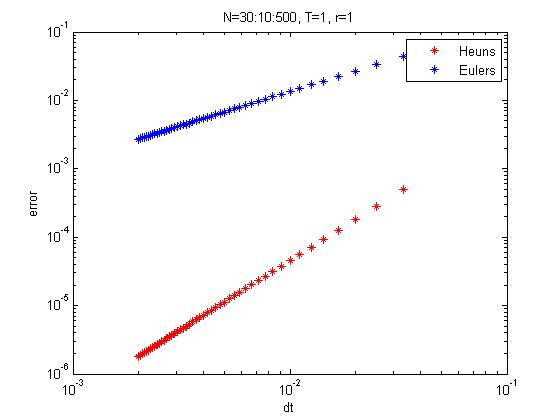
\includegraphics[width=6cm]{img/Heun500}
    histogram from Matlab simulations
    \column{.5\textwidth}
    %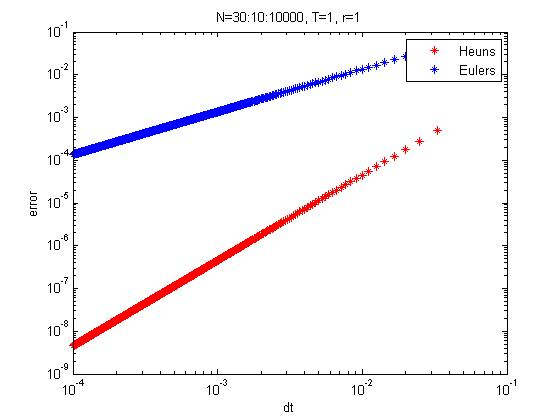
\includegraphics[width=6cm]{img/Heun10000}
    histogram from C simulations
  \end{columns}


\end{frame}



\subsection{Approximations}

\begin{frame}{Milstein Method}

	\begin{itemize}
		\item Technique for the approximate numerical solution of a stochastic differential equation
		\item Increases accuracy by using It\^o's Formula by adding the second-order term
	\end{itemize} 
	
	\vfill
	
Let $f_1(x_n,y_n) = f_1$, $g_1(x_n,y_n) = g_1$ and $W_1(x_n,y_n) = W_1$

		$$X_{n+1} = X_n + f_1\Delta t + g_1 \Delta W_1 + g_1 \frac{\partial g_1}{\partial x}  \cdot \left(\frac{1}{2} \Delta W_1 ^2 - \frac{1}{2} \Delta t \right)$$
	
	\vfill

\end{frame}

\begin{frame}{Full Approximations}
RESULTS \\
Because this is a random variable each time it's run it's different. \\
MOVIE INSERT 
\end{frame}

\begin{frame}{Confidence Intervals}
	
	\vfill
	
We wanted to better analyze our model so we found a $95\%$ confidence interval, for our Chi Square distribution. A confidence interval is a range of values (interval) that act as good estimates of the unknown population parameter. 
  
  $$\hat{\theta} - S(\hat{\theta}) L \leq \theta \leq \hat{\theta} + S(\hat{\theta}) L$$ \\
		Where $\hat{\theta}$ is the probability of each fixed point within the frequency table and
		$L$ is positive square root of the upper percentage point of the Chi Square distribution.
		
	\vfill
		
\end{frame}

\begin{frame}{Experimental Design}
To estimate the number of trials we solved the following formula for $n_1$, the number of trails corresponding to first fixed point, we have a total of $3$. \\
	
	\vfill

By letting $P_1 = \frac{1}{2}$ and $L = 5.991465$, we get:

  $$\sqrt{\frac{P_1 (1-P_1)}{n_1}} \ L = .01$$ \\
  $$n_1 = \frac{L^2 P_1 (1-P_1)}{.0001}$$ \\
  After multiplying by $3$ (our number of fixed points) we get: \\
  \begin{center} $N = 44935.9875$ \end{center} 

  From this we knew to run our programs $45,000$ times. 
	
\vfill

\end{frame}

\begin{frame}{Frequency Tables}

		Our frequency tables are divided into three fixed points:
\begin{itemize}
	\item species 1 lives while species 2 dies out, $n_1$
	\item species 2 lives while species 1 dies out, $n_2$
	\item species 1 and species 2 lives, $n_3$
\end{itemize}
\end{frame}


